In this section we will explain how to use the simulator and how it was used to influence the design of the robot. Finally some simulations will be shown.

\section{Simulation setup}
\begin{figure}[htp]
\center
    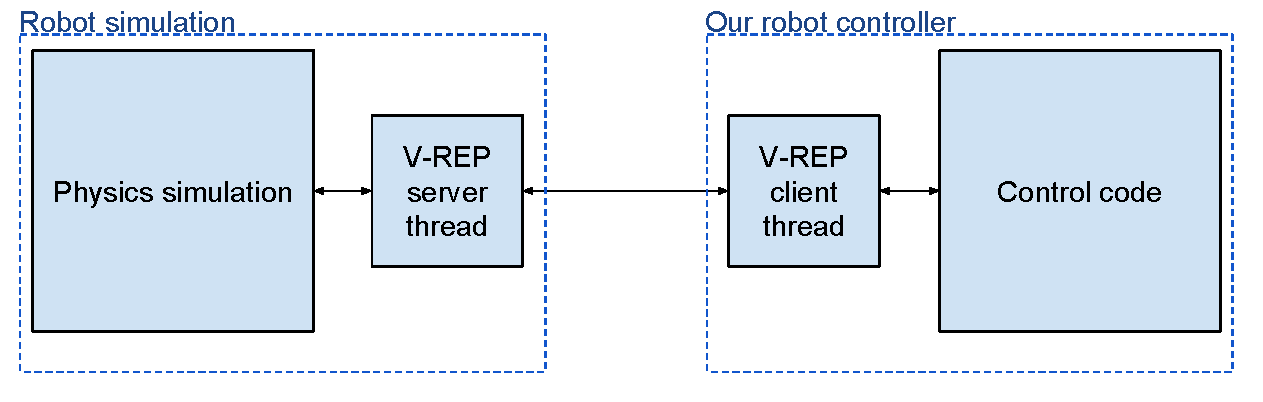
\includegraphics[width = 0.6\textwidth]{figures/simulation_principles}
    \caption{Schematic view of the simulation system. V-Rep handles solely the simulation of the robot and the control is established through a socket link with an external application which in our case is a MATLAB script.}
    \label{fig:simulation_principles}
\end{figure}

The architecture of the system is explained on \cref{fig:remoteApi}. We choose to operate in the synchronous operating mode : before V-REP simulates a timestep it waits for a trigger, allowing us to precisely control the robot.

\begin{figure}[htp]
\center
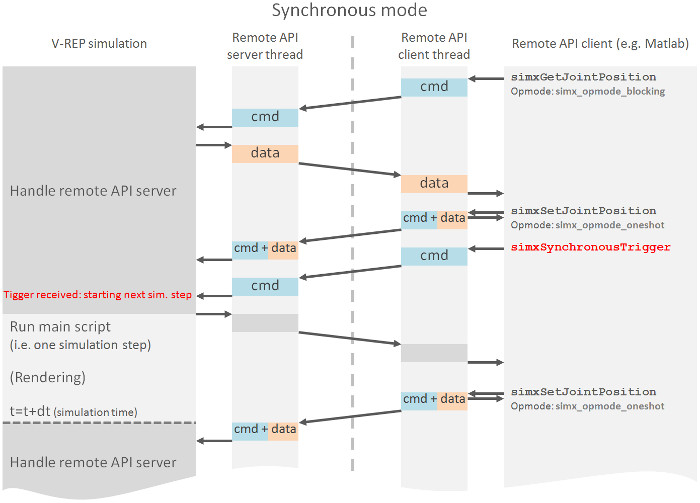
\includegraphics[width=0.6\textwidth]{figures/remoteApiSynchronous}
\caption[Simulation setup]{Explanation of the architecture of the simulation. The simulation runs on two threads : the simulation and the server thread. The server threads can receive orders from a client thread which is controlled by a custom application of our own.}
\label{fig:remoteApi}
\end{figure}

\section{Applications}
\subsection{Static stability}
\begin{table}[htp]
\center
\begin{tabularx}{\textwidth}{@{} X X X l @{}}
\toprule
\textbf{Module} & \textbf{Weight [$g$]} &  \textbf{Density [$kg/m^3$]}& \textbf{Dimensions [$mm \times mm \times mm$]}\\ 
\midrule
Odroid C-2 & 40 &  & 85.0 x 56.0 x 10.0\\
Li-Po battery & 188 & 2304 & 103.0 x 33.0 x 24.0\\
Mx-28R & 72 & 1150 & 35.6 x 50.6 x 35.5\\
LI-USB30-M021C & 22 & 2200 & 26.0 x 26.0 x 14.7\\
Frame Fr-07 & & 1200 & \\
Frame Fr-101-H3 & 7 & 1200 & \\
\bottomrule
\end{tabularx}
\caption[Weights and dimensions of the pieces of the robot]{Weights and dimensions of the pieces of the robot. The density is useful for the automatic computation of the weight and inertia of the pieces in V-REP.}
\label{table:weights}
\end{table}
\subsection{Standing up routines}
This section is heavily inspired by \cite{Stuckler06}

\subsection{Walking}

\section{Influence on robot's design}
The simulator helped shape the robot through simulations that unveiled serious design problems (inability to stand after a fall, inability to walk).

The final dimensions of the robot respect the rules of the contest:
\begin{itemize}
\item Height : $61.3cm$
\item Height of COM : $34cm$
\item Height of legs : $cm$
\item Height max is $< 1.5 \times 61.3$.
\item Foot area is $ cm^2$.
\end{itemize}